\chapter{GLOBAL MOTOR INVARIANT}
\label{chap:gi}


\nomenclature[a1]{$q$}{Generalized Coordinates}
\nomenclature[a2]{$\qd$}{Generalized Velocity}
\nomenclature[a3]{$\state$}{State Variable}
\nomenclature[a4]{$u$}{Control Input}
\nomenclature[a5]{$\mathrm{g}$}{Gravity}

\nomenclature[b1]{$Q$}{Configuration Space or Configuration Manifold}
\nomenclature[b2]{$TQ$}{Tangent Bundle of $Q$}
\nomenclature[b3]{$M$}{State Space Manifold}
\nomenclature[b4]{$TM$}{Tangent Bundle Manifold}



\nomenclature[c1]{$\mathcal{A}$}{Attractor}
\nomenclature[c2]{$\mathcal{B}(\mathcal{A})$}{Basin of Attraction of $\mathcal{A}$}
\nomenclature[c3]{$\simeq$}{Topology Conjungacy}



\nomenclature[d1]{$S$}{Neural Oscillator}
\nomenclature[d2]{$\uin$}{Input Signal to the Neural Oscillator}
\nomenclature[d3]{$\uout$}{Output of the Neural Oscillator}
\nomenclature[d4]{$\hin$}{Input Coefficient of the Neural Oscillator}
\nomenclature[d5]{$\hout$}{Output Coefficient of the Neural Oscillator}



%\nomenclature[zcif]{$CIF$}{Cauchy's Integral Formula}                                % first letter Z is for Acronyms 
%\nomenclature[aF]{$F$}{complex function}                                                   % first letter A is for Roman symbols
%\nomenclature[gp]{$\pi$}{ $\simeq 3.14\ldots$}                                             % first letter G is for Greek Symbols
%\nomenclature[gi]{$\iota$}{unit imaginary number $\sqrt{-1}$}                      % first letter G is for Greek Symbols
%\nomenclature[gg]{$\gamma$}{a simply closed curve on a complex plane}  % first letter G is for Greek Symbols
%\nomenclature[xi]{$\oint_\gamma$}{integration around a curve $\gamma$} % first letter X is for Other Symbols
%\nomenclature[rj]{$j$}{superscript index}                                                       % first letter R is for superscripts
%\nomenclature[s0]{$0$}{subscript index}                                                        % first letter S is for subscripts




\graphicspath{{GlobalInvariant/GlobalInvariantFigs/EPS/}{GlobalInvariant/GlobalInvariantFigs/}}


Motions are similar but vary greatly, for example, different people will walk with different gaits. 
A interesting question  is how the word ``walk'' refers to different gaits.
Motor Invariant Theory(\moit) proposes an answer:  despite differences in gaits, we agree on the word ``walk''  because in essence, we all walk in the same manner.
Intuitively, the gaits are periodic, energy efficient and stable.
The variations comes from the differences in body, environment or purpose, but from dynamic perspective, qualitatively, all the gaits dynamics share the same structure, or the qualitative properties of walking are invariant.
In \moit, the qualitative invariant properties are \emph{Global Motor Invariant}.


For biological perspective, we believe the walking ability is inborn and encoded in the body structure.
What ``Walk'' means is one motion primitive.
In \moit, motion primitive are identified by the global motor invariant.
Section~\ref{sec:GMIandMA} provides justification for the claim above in details.


In theory, it is difficult to define gait similarity mathematically.
Topology is introduce to for a clear definition of global invariant.
Such definition has important dynamic meaning, topologically equivalent means dynamic systems are qualitative the same.
Basic ideas of topology and qualitative dynamics are summarized at first in Section \ref{sec:qualiDy}

Entrainment are the biological based method to maintain global motor invariant, theory and experiment at discussed at the end of the chapter in Sections~\ref{sec:cpgcontrol} and Section~\ref{sec:qualyexample}







\section{Introduction to Qualitative Dynamics}
\label{sec:qualiDy}
Motion Primitives are ``trivial'' motion tasks.
Evolution equips animals with the body structure that animals can finish such tasks mainly by exploring the natural dynamics without too much control effort.
For dynamic perspective, the delicate design of body structure permit several patterns when interact with the living environment.  
Such patterns exists across detail variations in body structure (the tall and short characters) and environment (rough or plain ground).
Thus are robust or \emph{structural stable} in the dynamic term.
In \moit, identification of motion primitives and adaptation are based on the structural stability.
This section serve as a short introduction to concept idea and prepare mathematics.


Qualitative dynamic properties are analysed with the tool of differential topology.
This idea can be traced back to Poincare\citep{Poincar'e1899,Poincar'e1885} and recently developed by the Smale School\citep{Smale1970}.
There is no enough space to include the whole subject, please refer to book \citep{abraham1978foundations}for introduction in details.
Throughout this thesis,  geometrical perspective is adopted for it is more intuitive.
Some primary knowledge of topology and manifold is preferred and please refer to other dedicate sources for more accurate explanation. To make the thesis self-content, intuitive speaking,   \emph{topology} is the mathematical study of the properties that are preserved through deformations, twistings, and stretchings of objects. Tearing, however, is not allowed. A circle is topologically equivalent to an ellipse (into which it can be deformed by stretching) and a sphere is equivalent to an ellipsoid. And \emph{a manifold} is a topological space that on a small enough scale resembles the Euclidean space of a specific dimension.  A line and a circle are one-dimensional manifolds, a plane and sphere  are two-dimensional manifolds, and so on into high-dimensional space.


A dynamic system, usually described as a differential equation, from the geometrical perspective, describes a differentiable manifold.
Qualitative properties can be obtained by analysing the topological  property of geometry.
\emph{Global Motor Invariants} are identified by the topology structure.





\subsection{Dynamic Systems and Differentiable Manifold}
Motions of a mechanical system is determined by its configuration  $q$ in configuration space $Q$ and generalized speed $\qd$ in the tangent space $T_{q}Q$. 
Define the state value $\state=[q,\qd] \in M$,  $M$ is the state space, or state manifold.
A motion is a trajectory $t \mapsto q(t)$ in the configuration space parametrized by time~$t$.
For a dynamic system, $q(t)$ usually is derived from the state trajectory $\state(t)$, which is described by a differential equation. 



For every point $\state \in M$, 
$F$ and $u$ determines a derivative vector $\dot{\state}$ in the \emph{Tangent Space}~$T_{\state}M$. 
Vectors over the full space of $\state$ form the \emph{vector field} $\mathbf{V}$, described by a differential equation~ (Equation~\ref{eq:ode}.

\begin{equation}
\label{eq:ode}
\dot{\state}=F_{\alpha}(\state)+u
\end{equation}



where $u$ is the control effort. 
$\alpha$ is the system parameters
$F$ is determined by the system's natural property.
If $u=0$,  no control effort is applied.
Such systems are \emph{autonomous systems}. 

Solutions to Equation~\ref{eq:ode} is the \emph{integral curve}. 
\emph{Flow} $\Phi(\state)$ of $\mathbf{V}$ is the \emph{integral curve} through~$\state$. 
All the flows form the \emph{phase portrait}, which illustrates all the possible motions of the dynamic system.
Differential manifolds are usually visualized by \emph{phase plot}.

\textbf{Example}

For the mass-spring system, define state variable~$\state=[q,\qd]$, Equation~\ref{eq:mass-spring} can be transformed into the equation~\ref{eq:stateform}.
\begin{equation}
\label{eq:stateform}
\dot{\state}=
\left[ 
\begin{array}{cc}
0 &1\\
-1 &0 
\end{array}
\right]\state
\end{equation}



\subsection{Basin of Attraction}
Intersections of follows are \emph{equilibria}.
At each \textbf{equilibria}, the local space can be divided into subspaces: 
\emph{centre manifold}, \emph{stable manifold}, and \emph{unstable manifold}.
\begin{description} 
\item[centre manifold]
For a flow $\phi_c$ pass through a point $\state_{c}$ on centre sub manifold $W_{c}$, $\phi_c$ will remain on the Centre Manifold. 
\[
\phi_{c}(t) \in W_{c}, t \in R
\]

\item [stable manifold]
For a flow $\phi_{s}$ passes through a point $\state_{s}$ on stable sub manifold $W_{s}$, $\phi_s$ will finally converge to a flow $\phi_c$ on centre manifold.
\[
\phi_{s}(+\infty)=\phi_{c}
\]
\item[unstable manifold]
For a flow $\phi_u$ passes through a point $\state_u$ on unstable manifold $W_{u}$, $\phi_u$ will be repelled from the $\phi_c$ on centre manifold, the inverse of $\phi_u$ converges to $\phi_c$. 
\[
\phi_{u}(-\infty)=\phi_{c}
\] 
\end{description}


\textbf{Attractors} are the equilibriums where the whole local space is stable, the dimension of unstable manifold is zero.
\textbf{Repellors} are the equilibria where the whole local space is unstable,the dimension of stable manifold is zero.







In theory, only the attractors of the dynamic systems can be observed.
Two types of attractors are of great interest in motor control:
\begin{enumerate}
 \item Fixed Point, as show inf Figure~\ref{fig:StablePosture}.
 \item Limit Cycle,as shown in Figure~\ref{fig:ecycle}.
\end{enumerate}

\begin{figure}
	\begin{center}
	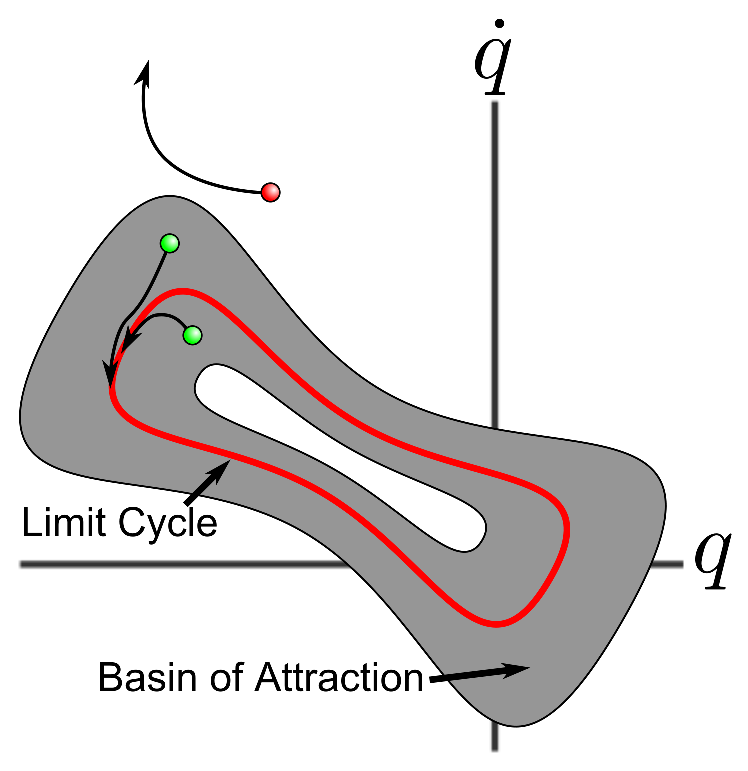
\includegraphics[height=0.4\textheight]{phase_plot}
	\end{center}
	\caption{Limit Cycle}
	\label{fig:ecycle}
\end{figure}





For non-linear dynamic systems, there may exist many attractors.
The phase plane will be divide into different regions,result in a cellular structure.
Within each region, all the flows will converge to one attractor ~$\mathcal{A}$.
The corresponding region is  the \emph{basin of attraction} ~$\mathcal{B}(\mathcal{A})$.

Figure~\ref{fig:manyboa} shown the landscape of phase portraits of a dynamic system.
\begin{figure}
\begin{center}
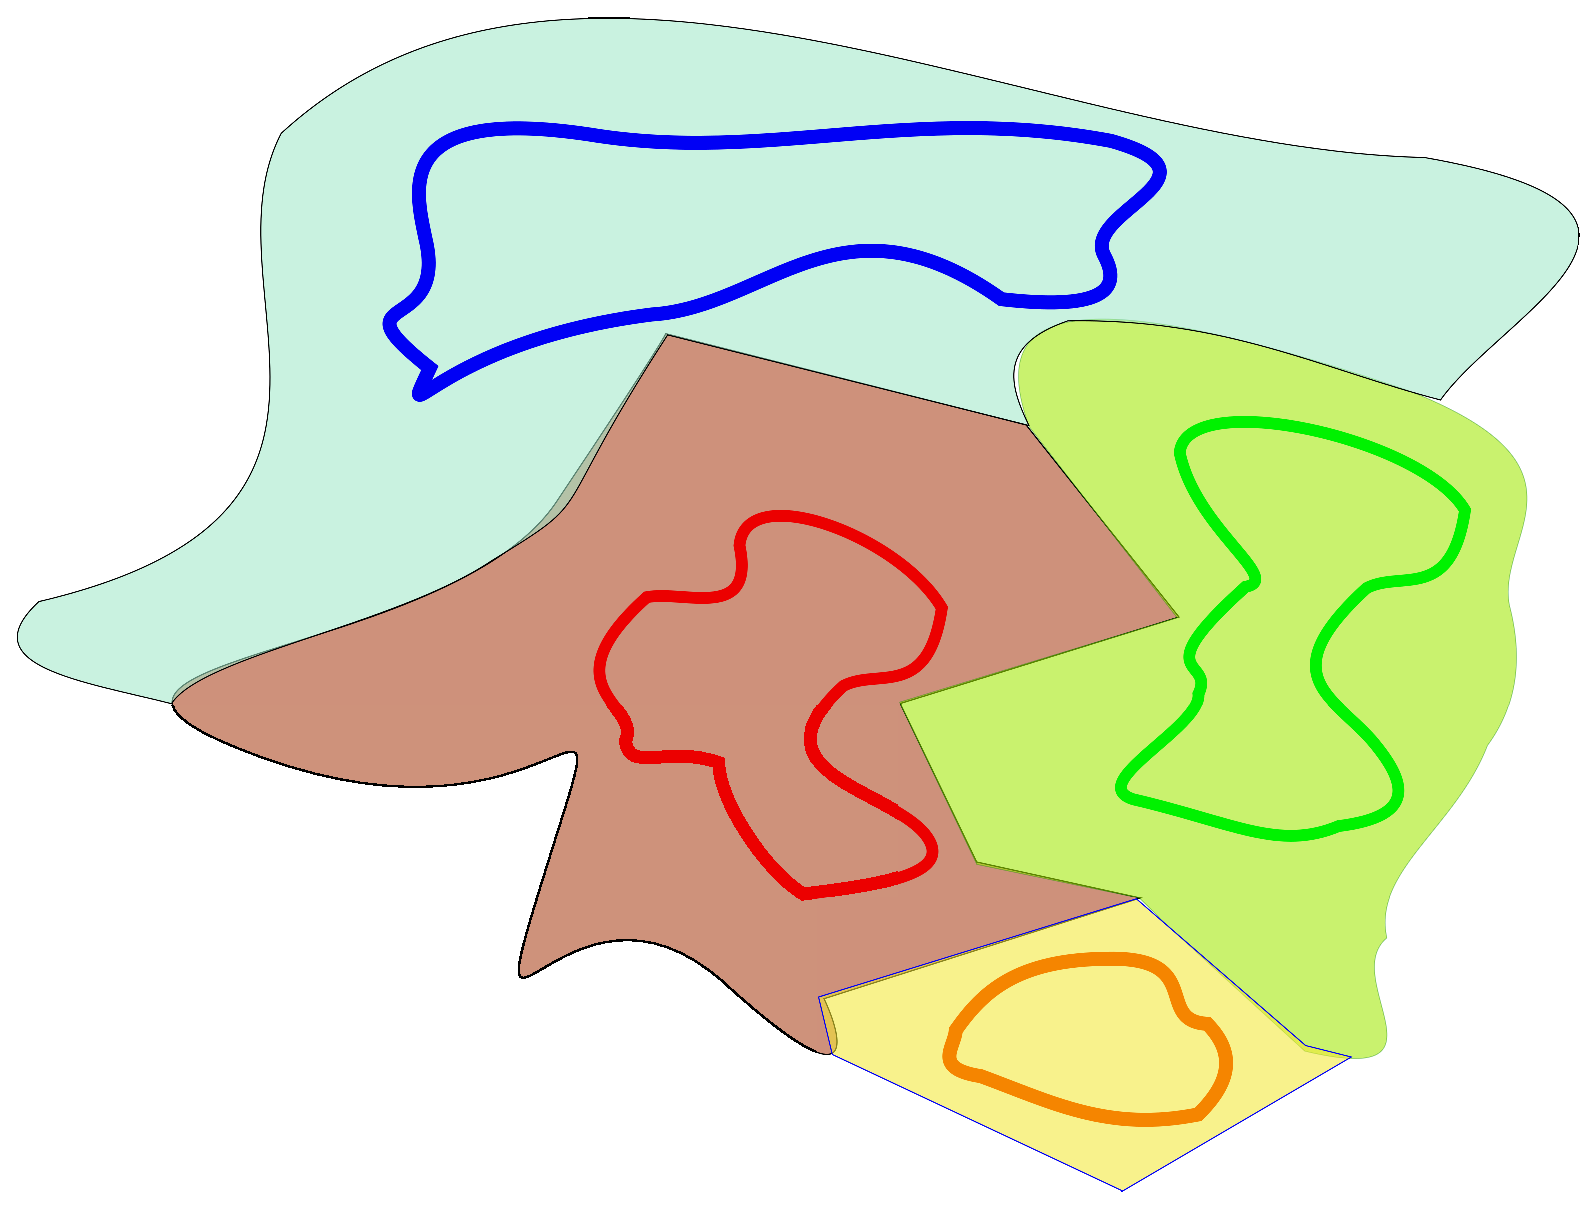
\includegraphics[height=0.4\textheight]{basinOfAttraction}
\end{center}
\caption{Cellular Structure of Phase Space}
\label{fig:manyboa}
\end{figure}




\subsection{Topology Conjugacy}
The topological structure of a dynamic system can be described by the type of equilibria and their connectivity.
Many dynamic systems have different dynamics but share the topology structure.
For example, the duffine system described by Equation ~\ref{eq:duffin} is different from the mass-spring system.
\begin{equation}
\label{eq:duffin}
\ddot{q}+q+q^{3}=0
\end{equation}

But the two system share the topology. 
Phase plot of the two system are show in Figure~\ref{fig:msphaseplot},\ref{fig:duffin}.
Flows of the two systems are similar, and we can ``deform '' one into another.
This equivalence relationship is called \emph{topological conjugacy}.

\begin{figure}
\begin{center}
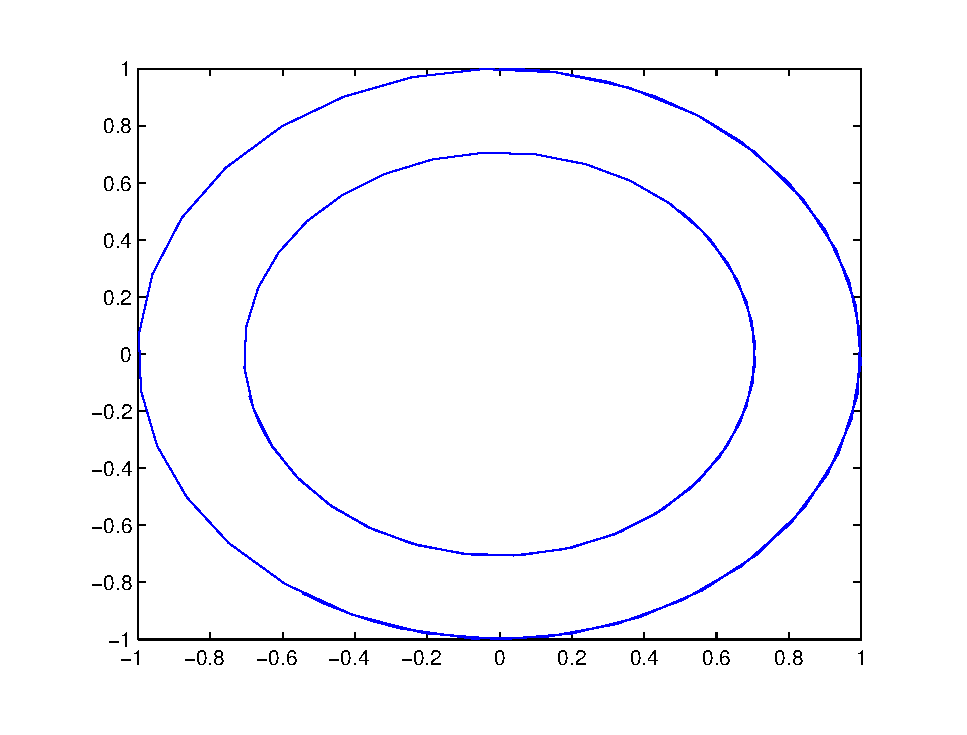
\includegraphics[height=0.4\textheight]{massspring}
\end{center}
\caption{Mass Spring System}
\label{fig:msphaseplot}
\end{figure}

\begin{figure}
\begin{center}
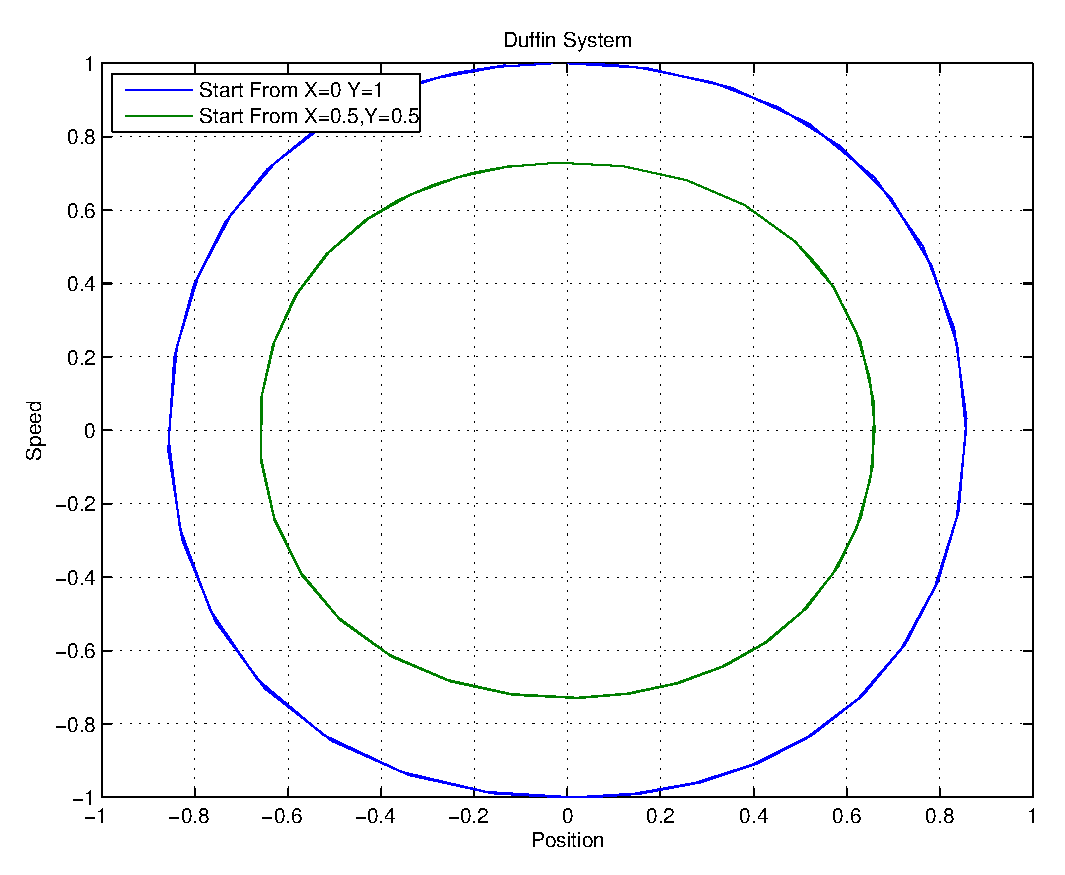
\includegraphics[height=0.4\textheight]{duffin}
\end{center}
\caption{Duffin Phase Plot}
\label{fig:duffin}
\end{figure}



\begin{mydef}
Let $M$ and $M'$ be topological spaces, and let $F\colon M\to M$ and $F'\colon M'\to M'$
be continuous functions. We say that $F$ is
\emph{topologically semi-conjugate} to $F'$, if there exists a continuous
surjection $S\colon M\to M'$ such that $FS=SF'$. If $S$ is a homomorphism,
then we say that $F$ and $F'$ are \emph{topologically conjugate}, and we call
$S$ a \emph{topological conjugation} between $F$ and $F'$.
if two system are topological conjugate, they are \emph{analogous systems}
\end{mydef}




\section{Global Motor Invariant and Motion Adaptation}
\label{sec:GMIandMA}
In \moit,  motion properties is determined by the attractors and basin of attractions of dynamics.
The `` trivial motion task'' of primitive rely on attractors.
If the attractor is fixed point, then the motion will be terminated.
if the attractor is limit cycle, then the motion will be periodic.

Larger basin of attraction means motion is more stable and narrow basin of attractions means the fragile stability.

\begin{mydef}
\emph{Global Motor Invariant} is the tuple of attractor and its basin of attraction
\end{mydef}


Motions vary because of different perturbations.
In \moit, perturbations are classified into category and coped with different control strategies.

\begin{itemize}
\HiItem{State perturbation}

Perturbations that only affect the state $\state$ are \emph{State Perturbations}.
State Perturbations change the current state, but not the underlying dynamic system.


If the perturbed state $\state'$ remains in the basin of attraction, the perturbed flow will converge to the same attractor. 
For the walking example, state perturbations can model the push and recover motion.

Different perturbations will result different flows and motions, the the final motion result will remain the same.
Such kind of motion adaptation is \emph{Responsive adaptation}.


To make the character more responsive without motion failure,
Motion controller should enlarge the basin of attraction.






\HiItem{Structure Perturbation}
Structure Perturbations affect the dynamic system.
For biological systems,  such kinds of perturbations are very common, when a man put a heavy box on his shoulder or injured, the dynamic will change, thus are structural Perturbation.


For some dynamic system,
Structural Perturbations may only deform the phase portrait and result in an analogous system.
Along with the phase portrait deformation, motion will vary but qualitative remain the same, this kind of motion adaptation is called \emph{system adaptation}.
For \cms, `` motion retargeting'' is a phenomenon of system adaptation.

Topological structure can not always maintained.
Some perturbations will result \emph{bifurcation} that the topology of the underlying dynamic system is changed.
As an  example is the damping perturbations on the mass spring system.
As show in Figure~\ref{fig:dampmass}

\begin{figure}
\begin{center}
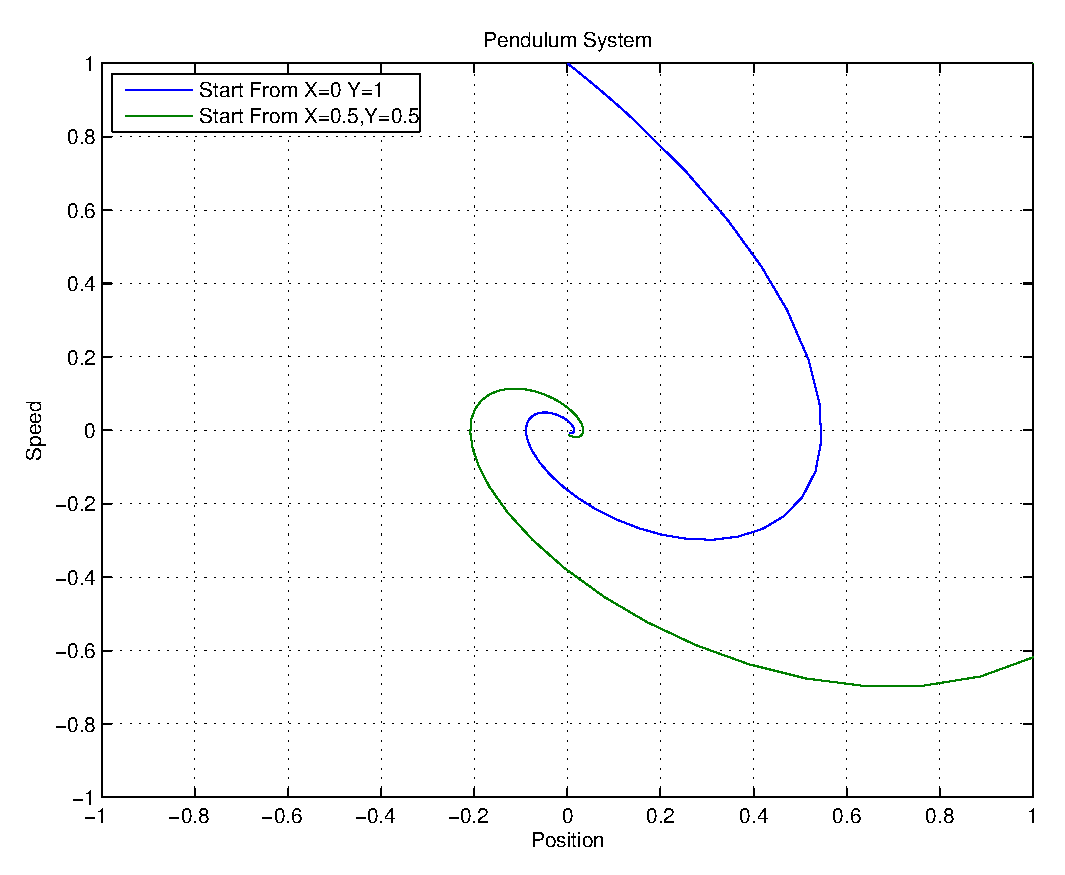
\includegraphics[height=0.4\textheight]{spring_damping}
\end{center}
\caption{damping perturbation on mass spring system}
\label{fig:dampmass}
\end{figure}

The ability of a dynamic system maintaining its topology structure is \emph{structural stability}.
To make characters more adaptive to environment and body change, motor controller should boost the structural stability of the motion.
Control effort are taken to prevent bifurcation.
\end{itemize}


\subsection{the biological meaning of Structural Stability}
\moit is a framework that unified many biological ideas.
For the  \umh,  the basin of attraction of an motion primitive can serve as the uncontrolled manifold of \umh.
State Perturbation are not controlled and motion is freely influence.
For \eph, attractor of motion primitive is a generalization of fix point.
Impedance control adjust the basin of attraction.


Structural Stability is new in \cms research, but there is a good reason for motor control to rely on it. 
In natural environment, perturbations and uncertainty are everywhere. 
Because of the sensing and computation limitations,  feedback idea  can't cope with all types of perturbations.
The alternative idea in motor invariant theory is  such perturbations can be neglected.
If the motion primitive is structural stable, even without control effort, motion will not change qualitatively.
Such an idea can reduce much of the computational burden and provide a framework for more types motion adaptation.


For some phenomena, structural stability and qualitative perspective provides a better explanation than optimization and feedback control.

Qualitative Control Theory may help to explain the  puzzle behind the  evolution of swimming and walking.
From quantitative perspective, the swimming dynamics are more difficult and walking should be easier.
While from the qualitative perspective, fluid is continuous and uniform, the dynamics is of simple topological structure is simple and stability is more easy to control.
Thus with little neural control fish can maintain its posture. 
On the other side, for human walking, although the rigid body dynamic are quantitative more easy, but topological structure of walking dynamics is much more complex. 
On the phase plane, there exist many equilibria and the basin of attraction of walking primitive has limited area,
thus the  stability of walking is fragile and needs more complex measures to enhance.

\moit also implies the similarity of the motion style for fish and wales
In spite of their different position on evolution chain, animals move through similar environment in a similar manner usually developed similar body structure.
The similarity in body structure promise the topological conjugacy and motions are based on the qualitative equivalent dynamics.
Also it reminded us motion primitive is close related to the environment, it is meaningless to talk about walking when put the character in deep water, even with the same control strategy, body and environment can not form the dynamics with desired topological structure.



Further \moit suggest the direction of evolution.
For one motion primitive, body may evolve to make the primitive more structural stable.






\section{Global Motor Invariant Control}
\label{sec:cpgcontrol}

In nature, the natural dynamics can be extremely complex. 
The corresponding manifolds has complex topological structure, which provides many motion primitives.
For \cms application, the question is whether different motion primitives can be controlled with a simple and unified method.
The idea is that even there are many types of motion primitives, the number of attractor type is limited. 
Also even the dimension of dynamic system is large, the dimension of the attractors is not. 
Basically there are only two types of attractors
\begin{itemize}
\item Fix point is of zero dimension. 
\item Limit cycle is of one dimension.
\end{itemize}

Control Strategy are designed based on the type of attractor.
For the fix point attractors, traditional \pd controllers are efficient.
While for the limit cycle attractors, the idea of entrainment is proposed.


\subsection{\cpg and Entrainment}
Biology Research suggested that the motor is mainly controlled by the Central Pattern Generator, which is a small autonomous network that generating rhythmic signals.
The idea of control motion by rhythmic signals can be modelled as entrainment \citep{Gonz'alez-Miranda2004}.
When coupling two oscillation system together, entrainment happens when two system oscillate in synchronize. 
This effect also known as resonant will enhance the oscillating behaviour. 




Mainly two types of attractors are observed : Fixed Point and Limited Cycle. 
In biological research, it is a still under hot debate which type attractor serve as the foundations for motor control\citep{Degallier2010}.
Current idea is that Limit Cycle is necessary, based on limit cycle, fix point can be achieved by
\begin{enumerate} 
\item terminate a cycle. 
\item approximated by a limit cycle with small amplitude.
\item Bifurcation. 
\end{enumerate}


In \moit, at current only the limit cycle is considered, mainly for two reasons: 
\begin{itemize}
\HiItem {periodic behaviour is  common} 
Besides the periodic motions such as swimming and running, other biological activity like heart beating, wake and sleep  are periodic.
A periodic system has the potential to integrate with other biological simulation.

\HiItem{similar results} 
For animations, periodic motions look similar to terminated motion when the amplitude of limit cycle is small. 
Thus if the oscillation amplitude can be controlled, both types of motion trajectories can be synthesized with one system.
\end{itemize}

\subsection{Neural Oscillator and its Stability}
For neural system, precise computation is difficult,  building oscillator with neurons is easy. 
Only two neurons are needed with mutual inhibitive property.
One extensively studied oscillation model is developed by \citet{neurooscillation}. 
The mathematical presentation is as follows:
\begin{align}
\tau_{1} \dot{s}_{1}&=c_1-s_{1}-c_2 l_{1}-c_3 [s_{2}]^{+}-\sum_{j}h_{ij}[w_{j}]^{+} \nonumber\\
\tau_{2} \dot{l}_{1}&=[s_{1}]^{+}-l_{1} \nonumber\\
\tau_{1} \dot{s}_{2}&=c_1-s_{2}-c_2 l_{2}-c_3 [s_{1}]^{-}-\sum_{j}h_{ij}[w_{j}]^{-} \nonumber\\
\tau_{2} \dot{l}_{2}&=[s_{2}]^{+}-l_{2}\label{eq:matsuta}
\end{align}
where $[t]^{+}=\max(0,t)$, $[t]^{-}=\min(0,t)$.
$c_1$,$c_2$,$c_3$ are parameters of the oscillator,in our research are kept constant$[c_1,c_2,c_3]=[1,2,2]$.
Values of $\tau_{1,2}$ controls the oscillation frequency, and their ratio controls the shape of wave.
In this research $\frac{\tau_{1}}{\tau_{2}}=0.5$


\begin{equation}
%y_{i}&=&\mbox{max}(s_{i},0)\\
\uout=\hout([s_{1}]^{+}-[s_{2}]^{+})
\end{equation}







Matuoka oscillator is an autonomous oscillator, which can start to oscillate without any control effort.
Figure ~\ref{fig:natural-oscilation} shows the natural oscillator output.
\begin{figure}[h]
\begin{center}
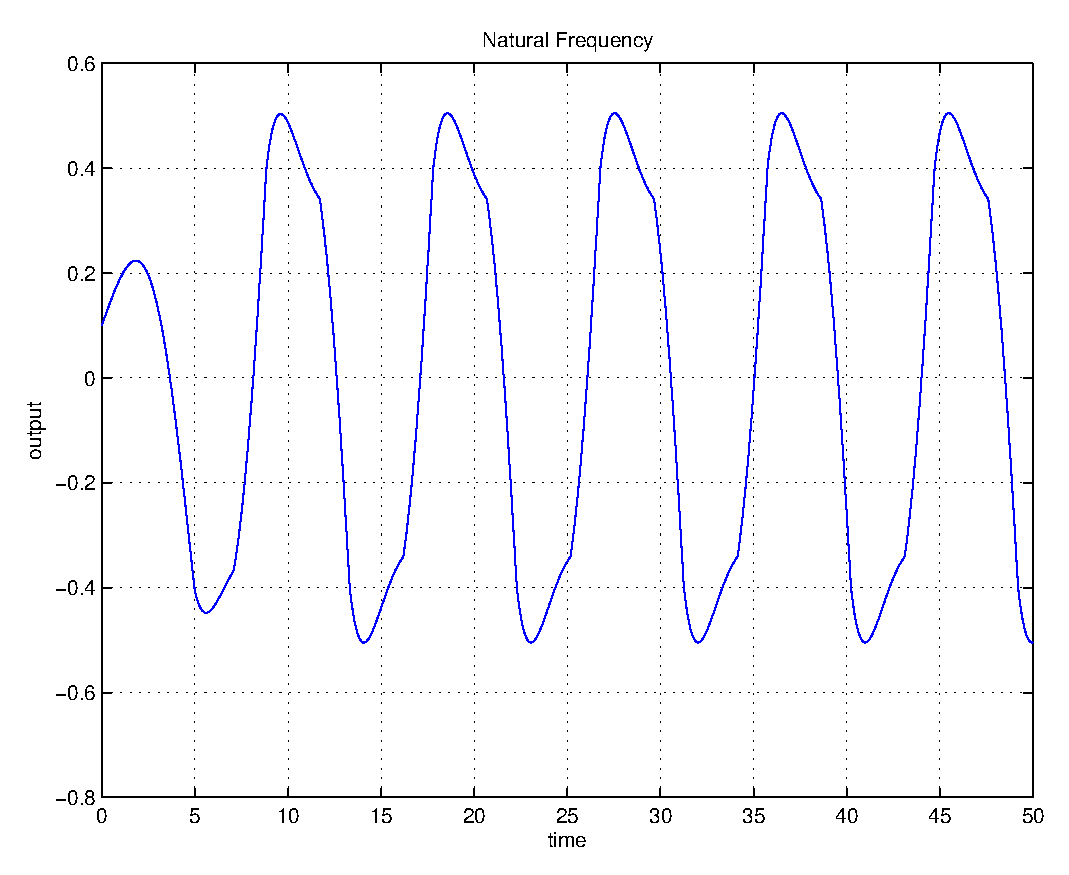
\includegraphics[height=0.4\textheight]{oscillation}
\caption{Natural Oscillation}
\label{fig:natural-oscilation}
\end{center}
\end{figure}





It is also adaptive; entrainment behaviour emerge between Matuoka oscillator and different oscillators. 
Figure~\ref{fig:entraint-oscilation} shows the entrainment oscillation,where  Matuoka oscillator synchronise with the input signal.
\begin{figure}[h]
\begin{center}
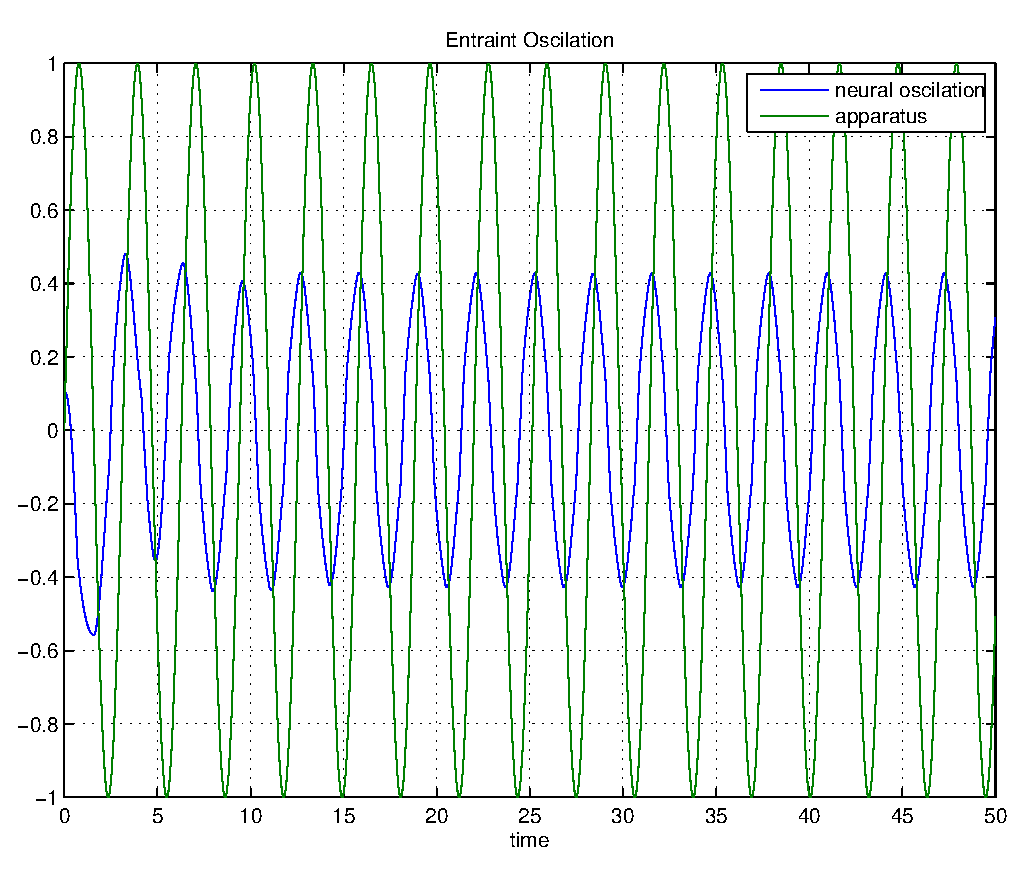
\includegraphics[height=0.4\textheight]{entraint_oscilation}
\caption{Entrainment Oscillation}
\label{fig:entraint-oscilation}
\end{center}
\end{figure}

Because of the nonlinear properties, behaviour of Matsuoka Oscilator is not completely understood. 
Matsuta\citep{Matsuoka1987} analyze the adaptive properties by investigating the location of the roots of characteristic equation. 
Wilimas\citep{Williamson1998} analyze the properties in frequency domain.
This research investigates the qualitative property by analyzing the topology of  empirical results.
The Matsuoka Oscillator shows three important properties:
\begin{itemize}
\item{Simple Topological Structure.}
The topology structure of neural oscillator is simple, 
it includes one  attractive limit circle and one fix repellor.
\item{Large Basin of Attraction.}
All the simulations we carried out converged to the same limited circle.
\item{Fast Converging Speed.}
In most of the case, the flow will converge to the limit circle within one period time.
\end{itemize}






Features above are shown in Figure ~\ref{fig:time_timeAttraction}.
\begin{figure}
\begin{center}
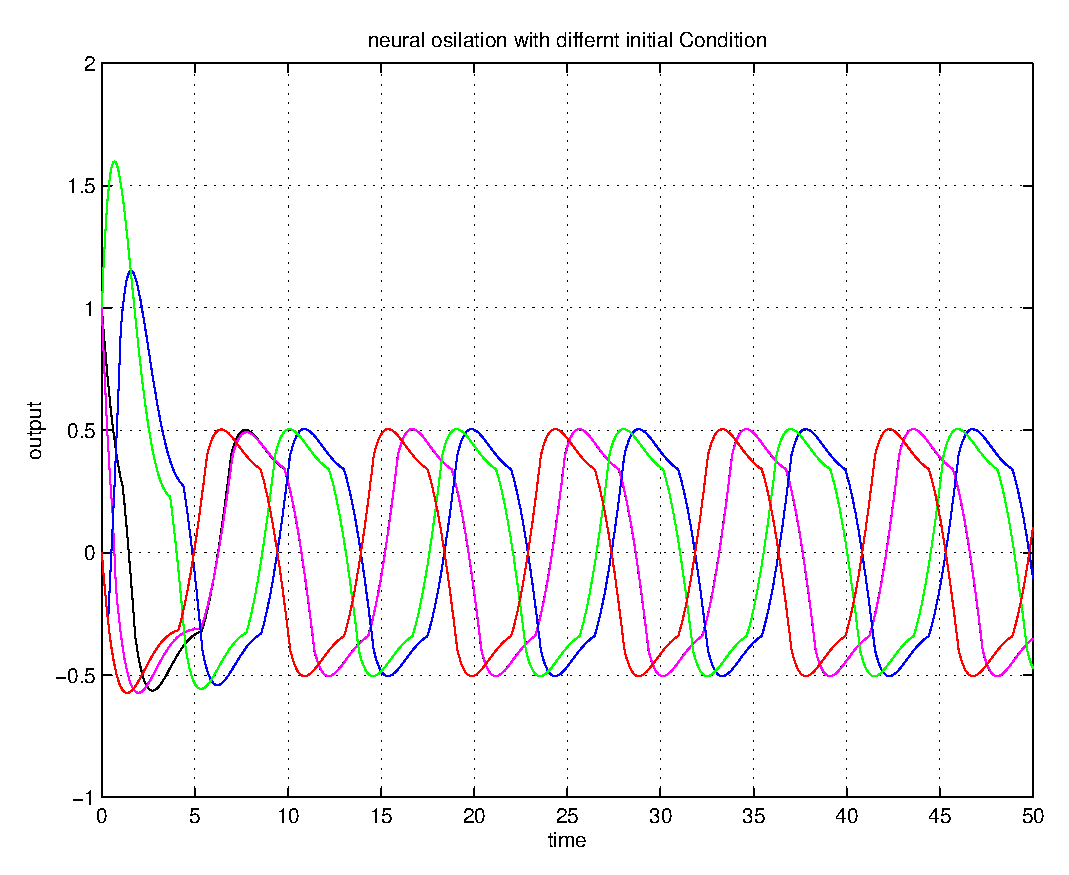
\includegraphics[height=0.4\textheight]{neural_attraction}
\end{center}
\caption{Neural output with different initial position}
\label{fig:time_timeAttraction}
\end{figure}

\begin{figure}
\begin{center}
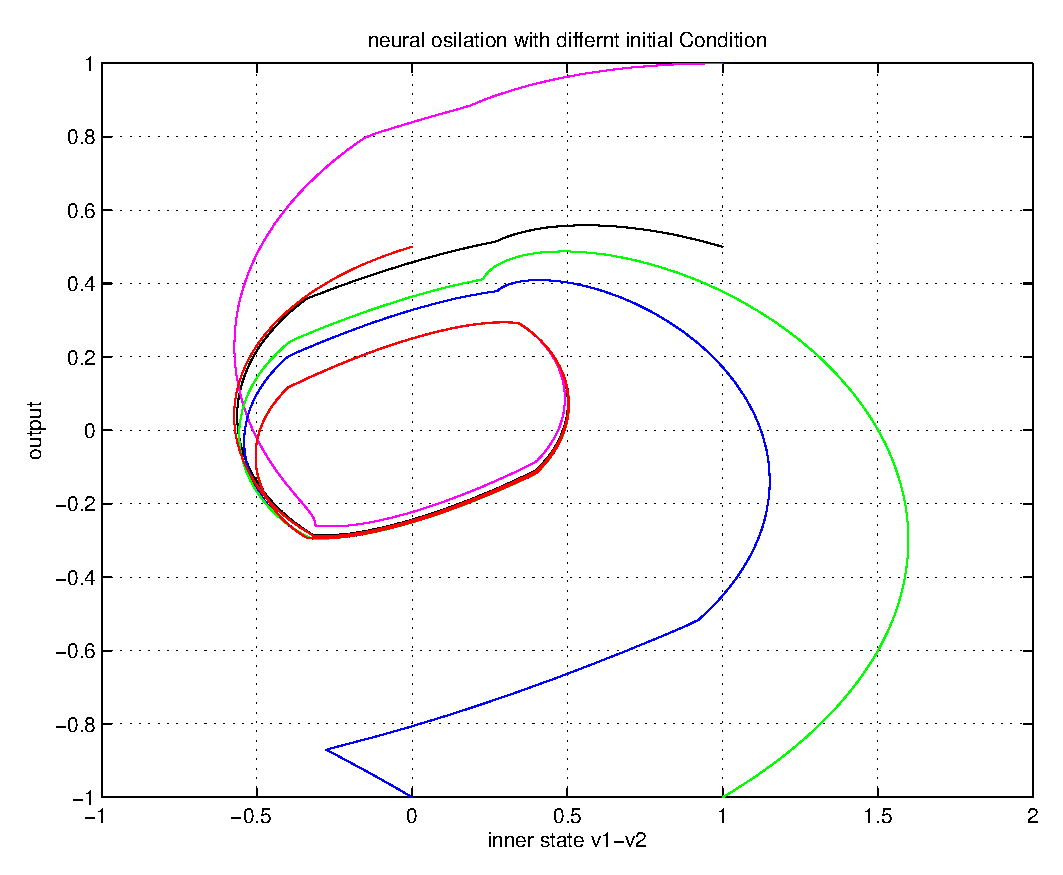
\includegraphics[height=0.4\textheight]{neural_attraction_phase}
\end{center}
\caption{Phase plot of oscillation with different initial condition}
\label{fig:phase_attraction}
\end{figure}
 
The large area of basin of attraction means the final behaviour is totally determined by system parameters. 
Initial condition will have no effects on the stable oscillation behaviour. 
Matsuta oscillator can be treated as single input, single output system.
The output signal is controlled by three system parameters and input signal. 
Equation ~\ref{eq:matsuta} can be reformed in the form of Equation~\ref{eq:simplematsuta}.
\begin{equation}
\label{eq:simplematsuta}
\uout=S_{[\hin,\hout,\tau]}(\uin)
\end{equation}
where $\uin=\sum_{j}h_{j}[w_{j}]=hw$.





The converging speed can be seen as quick recovery ability.
When an impulse perturbation happens, it will recover in one period time.


\section{Example:Maintain Ball Bouncing Height}
\label{sec:qualyexample}
The Bouncing Ball system is shown in Figure~\ref{fig:bball}, where a ball is bouncing on a moving paddle.
The dynamics of this system is simple, but difficult to control with optimization or \pd methods.
\begin{figure}
\begin{center}
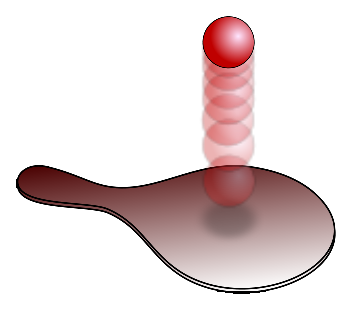
\includegraphics[height=0.4\textheight]{paddleball}
\end{center}
\caption{The Bouncing Ball System}
\label{fig:bball}
\end{figure}
 
The bouncing ball system captures the complex discontinuous dynamics when human iteract with the environment and object. 
It can be the basic model for many motion tasks like jumping, running and ball playing.
This example demostrates how limit cycle are generate through neural  oscillator entrainment.
 
\subsection*{Dynamics}
The dynamics of the bouncing ball system is hybrid, it involves two phases.
\begin{itemize}
\HiItem{The Flying Phase}
When the ball is flying, it is only affected by the gravity.
\HiItem{The Strike Phase}
When the ball hit the paddle, the speed of the ball is changed instantly.
\end{itemize}
The natural dynamics of bouncing ball system are described by  Equation~\ref{eq:bbeq},and are shown by Figure~\ref{fig:bborg}. 
The ball will  bounce with ever smaller height. 

\begin{align}
\label{eq:bbeq}
\ddot{q}_{ball}&=-g&\mathrm{if}\,\,q_{ball} &> q_{paddle}\,\,\mathrm{(free\,\,flying)} \nonumber\\
\dot{q}^{+}_{\mathrm{ball}} - \dot{q}^{+}_{\mathrm{paddle}} &=  \epsilon(\dot{q}^{-}_{\mathrm{ball}} - \dot{q}^{-}_{\mathrm{paddle}})&\mathrm{if}\,\,q_{ball} &\leq {q_{paddle}}\,\,\mathrm{(paddle\,\,strike)}\nonumber
\end{align}



\begin{figure}[h]
\begin{center}
	\subfigure[state plot]
	{
	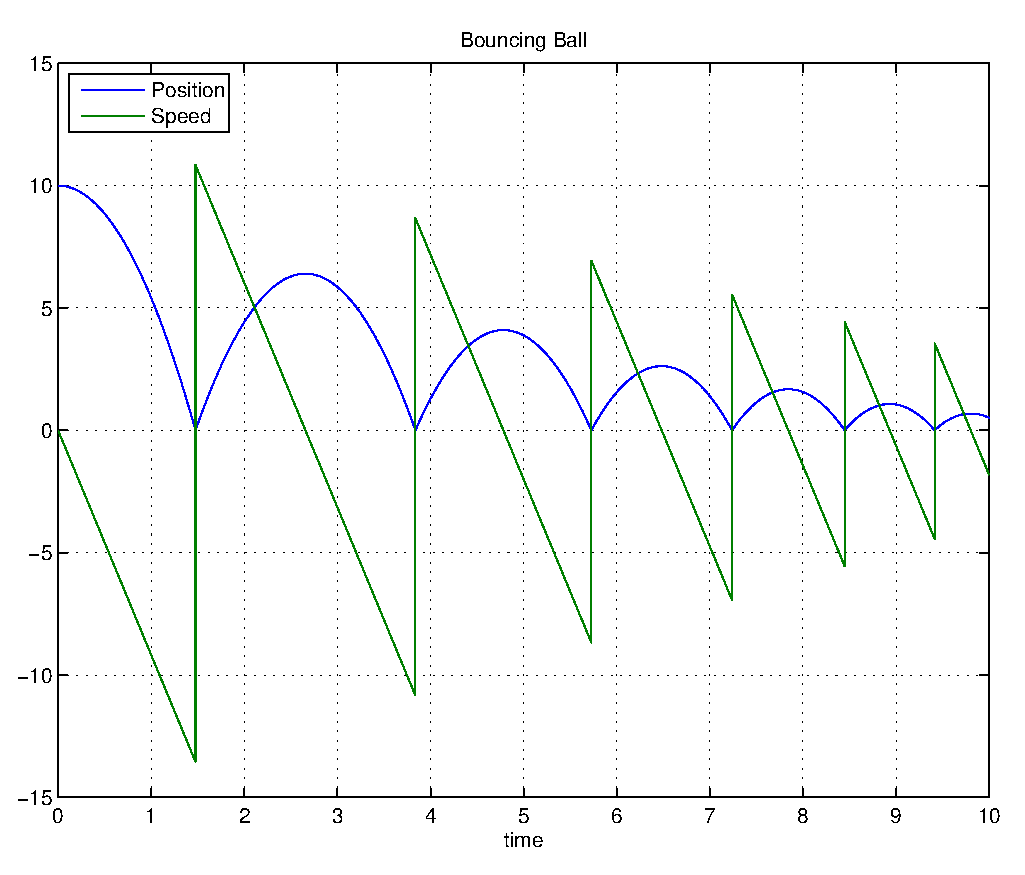
\includegraphics[width=0.45\textwidth]{bouncing_ball}
	\label{fig:bb}
	}
	\subfigure[Phase Plane]
	{
	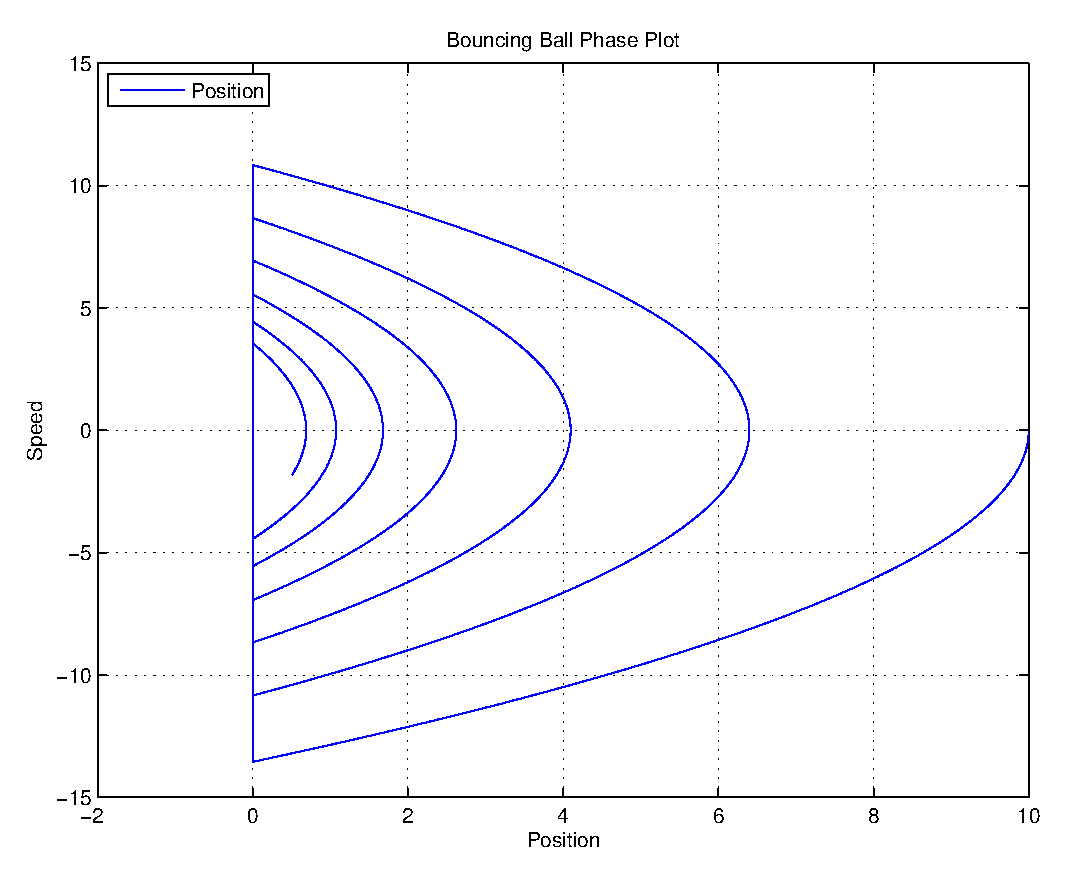
\includegraphics[width=0.45\textwidth]{bouncing_ball_phaseplot}
	\label{fig:bbp}
	}
	
\end{center}
\caption{Original Bourncing Ball System}
\label{fig:bborg}
\end{figure}



\subsection*{Emergence of Limit Cycle}
The autonomous system of bouncing ball has only one fixed point attractor and its basin of attraction covers the whole phase space.
The bouncing ball shows the near periodic behaviour, thus can be seen as bifurcation of some periodic ones.
Neural Oscillator can be applied to maintain the original periodic motion, and limit cycle emerges from entrainment.
The input of neural oscillator is the velocity $\uin=\qd_{ball}$, the output drives the paddle position $q_{paddle}=\uout$.
Dropped from different position, all the ball will bouncing  about the same height of $5 unit$,as show in Figure~\ref{fig:bb_attractive_circle}.
The bouncing height can be maintained.

\begin{figure}[h]
\begin{center}
	\subfigure[State Plot]
	{
	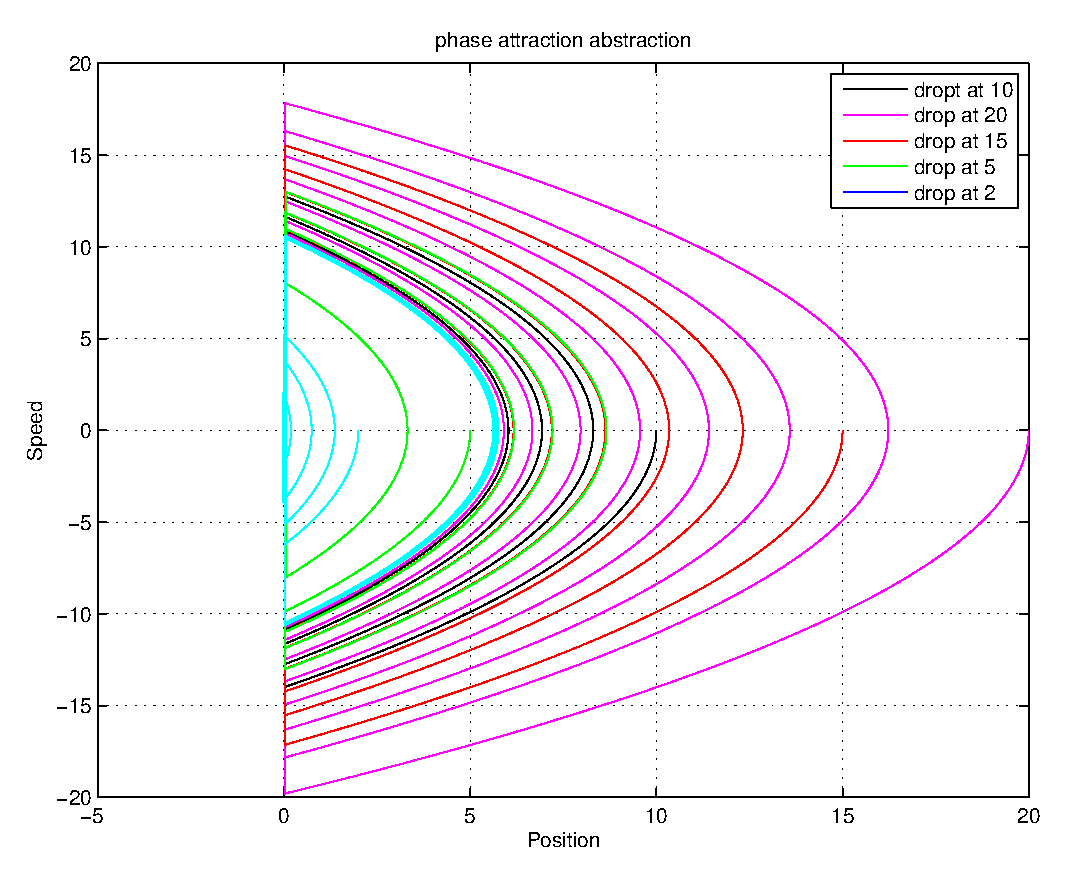
\includegraphics[width=0.45\textwidth]{bb_ms_os_attraction_phase}
	\label{fig:bb_attractive_entraint}
	}
	\subfigure[Phase Plane]
	{
	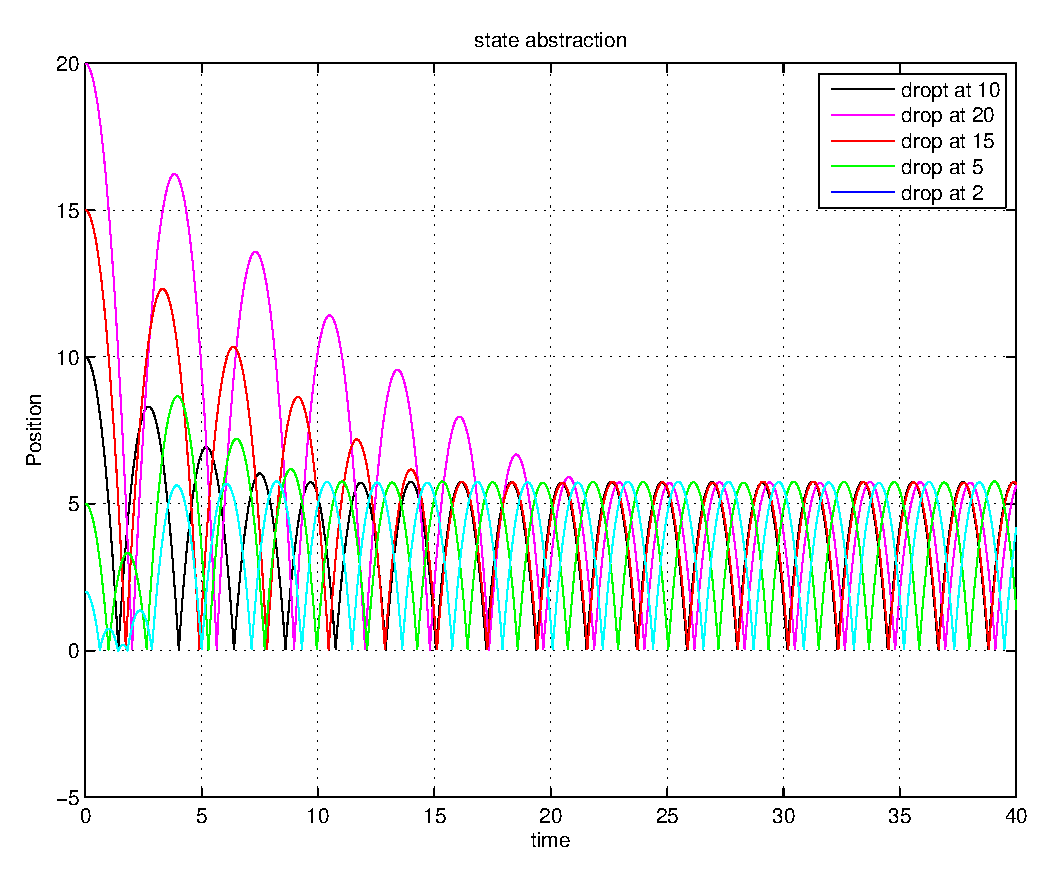
\includegraphics[width=0.45\textwidth]{bb_ms_os_StateTimeAttraction}
	\label{fig:bb_attractive_entraint_time}
	}
	
\end{center}
\caption{Attractive Limited Circle}
\label{fig:bb_attractive_circle}
\end{figure}

